\subsection{Further properties of inner product spaces}


\begin{exercise}{2}
Give examples of subspaces of $l^2$
\end{exercise}
\begin{proof}
\begin{enumerate}
    \item $l^2$ itself.
    \item The set $\set{0}$.
    \item The space of sequences with finitely many nonzero elements.
    \item The set $\set{(x,x/2,x/3,\dots): x\in\R}$.
\end{enumerate}
\end{proof}

\begin{exercise}{4}
Show that $y\perp x_n$ and $x_n\to x$ together imply $x\perp y$.
\end{exercise}
\begin{proof}
We have
\begin{align*}
    \absoluteValue{\brackets{x,y}}
    =& \absoluteValue{\brackets{x+x_n-x_n,y}}\\
    =& \absoluteValue{\brackets{x-x_n,y} + \brackets{x_n,y}}\\
    =& \absoluteValue{\brackets{x-x_n,y}}\\
    \leq& \norm{x-x_n}\norm{y}\to 0.
\end{align*}
Where the third equality holds because $\brackets{x_n,y}=0$ for all $x_n$, the inequality follows from the Cauchy-Schwarz inequality, and the convergence to 0 follows from the fact that $\norm{y}$ is fixed, but $x_n\to x$, so that $\norm{x_n-x}\to 0$.
\end{proof}

\begin{exercise}{5}
Show that for a sequence $(x_n)$ in an inner product space the conditions $\norm{x_n}\to\norm{x}$ and $\brackets{x_n,x}\to\brackets{x,x}$ imply convergence $x_n\to x$.
\end{exercise}
\begin{proof}
We have
\begin{align*}
    \norm{x_n-x}^2
    =& \brackets{x_n-x, x_n-x}\\
    =& \brackets{x_n,x_n-x} - \brackets{x,x_n-x}\\
    =& \overline{\brackets{x_n-x,x_n}} - \overline{\brackets{x_n-x,x}}\\
    =& \overline{\brackets{x_n,x_n}} -\overline{\brackets{x,x_n}} - \overline{\brackets{x_n,x}} + \overline{\brackets{x,x}}\\
    =& \norm{x_n}^2 -\overline{\brackets{x,x_n}} - \overline{\brackets{x_n,x}} + \norm{x}^2\\
    \to& \norm{x}^2 -\overline{\brackets{x,x}} - \overline{\brackets{x,x}} + \norm{x}^2\\
    =& \norm{x}^2 - \norm{x}^2 - \norm{x}^2 + \norm{x}^2 = 0,
\end{align*}
as required.
\end{proof}

\begin{exercise}{7}
Show that in an inner product space, $x\perp y$ if and only if we have $\norm{x+ay} = \norm{x-ay}$ for all scalars $a$.

\begin{figure}[H]
    \centering
    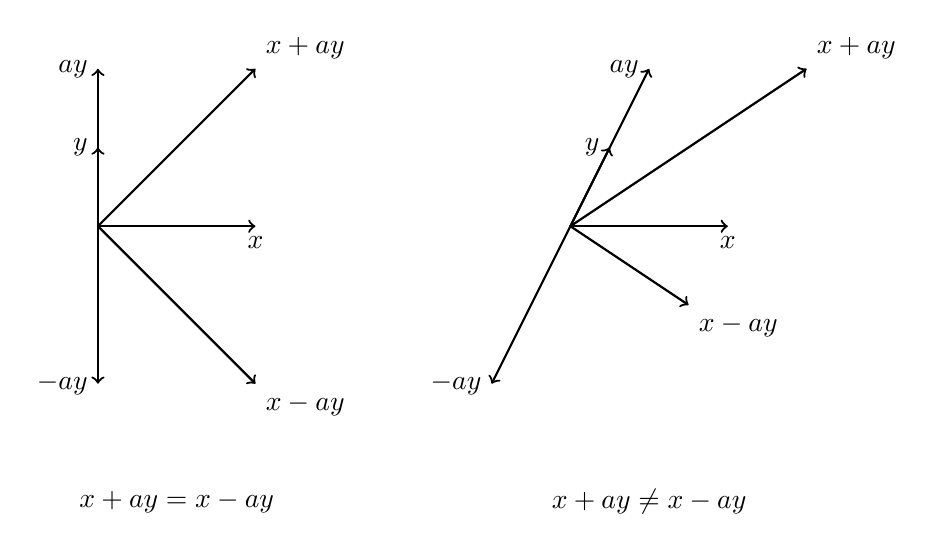
\begin{tikzpicture}
    % Left Diagram
    \draw[thick,->] (0,0) -- (2,0) node[below] {$x$};
    \draw[thick,->] (0,0) -- (0,1) node[left] {$y$};
    \draw[thick,->] (0,0) -- (0,2) node[left] {$a y$};
    \draw[thick,->] (0,0) -- (0,-2) node[left] {$-a y$};
    \draw[thick,->] (0,0) -- (2,2) node[above right] {$x + a y$};
    \draw[thick,->] (0,0) -- (2,-2) node[below right] {$x - a y$};
    
    % Right Diagram
    \begin{scope}[xshift=6cm]
        \draw[thick,->] (0,0) -- (2,0) node[below] {$x$};
        \draw[thick,->] (0,0) -- (.5,1) node[left] {$y$};
        \draw[thick,->] (0,0) -- (1,2) node[left] {$a y$};
        \draw[thick,->] (0,0) -- (-1,-2) node[left] {$-a y$};
        \draw[thick,->] (0,0) -- (3,2) node[above right] {$x + a y$};
        \draw[thick,->] (0,0) -- (1.5,-1) node[below right] {$x - a y$};

    \end{scope}
    
    % Bottom equations
    \node at (1,-3.5) {$\norm{x + ay} = \norm{x - a y}$};
    \node at (7,-3.5) {$\norm{x + a y} \neq \norm{x - a y}$};
\end{tikzpicture}
    \caption{Illustration of the exercise 7 in the Euclidean plane $\R^2$}
    \label{fig:sec3-1-ex7}
\end{figure}
\end{exercise}
\begin{proof}
($\Rightarrow$)
Suppose $x\perp y$, we then have
\begin{align*}
    \norm{x+ay}^2
    =& \brackets{x+ay, x+ay}\\
    =& \brackets{x, x+ay} + a\brackets{y,x+ay}\\
    =& \overline{\brackets{x+ay, x}} + a\overline{\brackets{x+ay,y}}\\
    =& \overline{\brackets{x, x}} + \overline{a\brackets{y, x}}
    + a\overline{\brackets{x,y}} + a\bar{a}\overline{\brackets{y,y}}\\
    =& \norm{x}^2 + \overline{a\brackets{y, x}}
    + a\overline{\brackets{x,y}} + a\bar{a}\norm{y}^2.
\end{align*}
Furthermore,
\begin{align*}
    \norm{x-ay}^2
    =& \brackets{x-ay, x-ay}\\
    =& \brackets{x, x-ay} - a\brackets{y,x-ay}\\
    =& \overline{\brackets{x-ay, x}} - a\overline{\brackets{x-ay,y}}\\
    =& \overline{\brackets{x, x}} - \overline{a\brackets{y, x}}
    - a\overline{\brackets{x,y}} + a\bar{a}\overline{\brackets{y,y}}\\
    =& \norm{x}^2 - \overline{a\brackets{y, x}}
    - a\overline{\brackets{x,y}} + a\bar{a}\norm{y}^2.
\end{align*}
Since we assume $x\perp y$, then $\brackets{x,y}$ $\brackets{y,x}$ are both 0 and we get the desired equality.

($\Leftarrow$)
Suppose $\norm{x+ay} =\norm{x-ay}$ holds for all $a$.
Using the above results, we have
\begin{align*}
    &\norm{x+ay}^2 = \norm{x-ay}^2 &&\iff\\
    &\norm{x}^2 + \overline{a\brackets{y, x}}
    + a\overline{\brackets{x,y}} + a\bar{a}\norm{y}^2 
    = \norm{x}^2 - \overline{a\brackets{y, x}}
    - a\overline{\brackets{x,y}} + a\bar{a}\norm{y}^2 &&\iff\\
    &\overline{a\brackets{y, x}}
    + a\overline{\brackets{x,y}}
    = - \overline{a\brackets{y, x}}
    - a\overline{\brackets{x,y}} &&\iff\\
    &\overline{a\brackets{y, x}}
    = -a\overline{\brackets{x,y}}.
\end{align*}
Since the equality holds for all $a$, choose $a/\bar{a}=\overline{\brackets{y,x}}/\overline{\brackets{x,y}}$ to get $2\overline{\brackets{y,x}}=0$, which holds only if $\brackets{x,y}=0$, that is $x\perp y$.
\end{proof}

\begin{exercise}{8}
Show that in an inner product space, $x\perp y$ if and only if $\norm{x+ay}\geq\norm{x}$ for all scalars $a$.
\end{exercise}
\begin{proof}
($\Rightarrow$)
From the previous exercise, we have
\begin{align*}
    \norm{x+ay}^2
    =& \brackets{x+ay, x+ay}\\
    =& \norm{x}^2 + \overline{a\brackets{y, x}}
    + a\overline{\brackets{x,y}} + a\bar{a}\norm{y}^2,
\end{align*}
so that if $\brackets{x,y}$ and $\brackets{y,x}$ are both 0, then $\norm{x+ay}^2 =\norm{x}^2+\absoluteValue{a}\norm{y}^2 \geq\norm{x}^2$, as required.

($\Leftarrow$)
On the other hand, if the inequality holds for all $a$, we will first assume $a$ is real to obtain
\begin{align*}
    &\norm{x+ay}^2
    \geq \norm{x}^2\\
    &\brackets{x+ay, x+ay}
    \geq \norm{x}^2 &&\iff\\
    &\norm{x}^2 + \overline{a\brackets{y, x}}
    + a\overline{\brackets{x,y}} + a\bar{a}\norm{y}^2
    \geq \norm{x}^2 &&\iff\\
    &\overline{a\brackets{y, x}}
    + a\overline{\brackets{x,y}} + a\bar{a}\norm{y}^2
    \geq 0 &&\iff\\
    &\absoluteValue{a}^2\norm{y}^2 + 2\text{Re}(a\brackets{y, x})
    \geq 0 &&\iff\\
    &\absoluteValue{a}^2\norm{y}^2 + 2a\text{Re}(\brackets{y, x}) \geq 0.
\end{align*}
We will now analyse the case where $a$ is positive and the case where $a$ is negative.
If $a$ is positive, then 
$a\geq -2\text{Re}(\brackets{y,x})/\norm{y}^2$, so that $a\leq 2\text{Re}(\brackets{y,x})/\norm{y}^2$
If $a$ is negative, then
$a\geq 2\text{Re}(\brackets{y,x})/\norm{y}^2$.
If we let $a\to 0$, we get that $0\leq\text{Re}(\brackets{y,x})$ and $0\geq\text{Re}(\brackets{y,x})$.
That is $\text{Re}(\brackets{y,x})=0$.

If we assume $a$ is imaginary, say $a=ib$ where $b$ is real, then
\begin{align*}
    &\norm{x+ay}^2
    \geq \norm{x}^2\\
    &\brackets{x+ay, x+ay}
    \geq \norm{x}^2 &&\iff\\
    &\norm{x}^2 + \overline{a\brackets{y, x}}
    + a\overline{\brackets{x,y}} + a\bar{a}\norm{y}^2
    \geq \norm{x}^2 &&\iff\\
    &\overline{bi\brackets{y, x}}
    + bi\overline{\brackets{x,y}} + bi\bar{bi}\norm{y}^2
    \geq 0 &&\iff\\
    &-bi\overline{\brackets{y, x}}
    + bi\overline{\brackets{x,y}} + bi\bar{bi}\norm{y}^2
    \geq 0 &&\iff\\
    &\absoluteValue{b}^2\norm{y}^2 + 2\text{Im}(b\brackets{y, x})
    \geq 0 &&\iff\\
    &\absoluteValue{b}^2\norm{y}^2 + 2b\text{Im}(\brackets{y, x}) \geq 0.
\end{align*}

We can analyse, mutatis mutandis, the same cases with $b$ being positive and negative to conclude that $\text{Im}(\brackets{y,x})=0$, so that $\brackets{y,x}=0$ giving us $x\perp y$, as required.
\end{proof}

\begin{exercise}{10 (Zero operator)}
Let $T:X\to X$ be a bounded linear operator on a complex inner product space $X$.
If $\brackets{Tx,x}=0$ for all $x\in X$, show that $T=0$.

Show that this does not hold in the case of a real inner product space.
Hint: Consider a rotation of the euclidean space.
\end{exercise}
\begin{proof}
This was proven in Axler 7.14, I reproduce the proof here, almost verbatim but developing where there were missing steps.
We have
\begin{align*}
    \brackets{Tu,w} 
    =& \frac{\brackets{T(u+w), u+w}-\brackets{T(u-w), u-w}}{4}\\
    +& \frac{\brackets{T(u+iw), u+iw}-\brackets{T(u-iw), u-iw}}{4}i.
\end{align*}
To see this, first consider the first summand on the right hand side
\begin{align*}
    &\frac{\brackets{T(u+w), u+w} - \brackets{T(u-w), u-w}}{4}\\
    =& \frac{\brackets{Tu, u+w} + \brackets{Tw, u+w}}{4}\\
    &-\frac{\brackets{Tu, u-w} + \brackets{Tw, u-w}}{4}\\
    =& \frac{\overline{\brackets{u+w,Tu}} + \overline{\brackets{u+w,Tw}}}{4}\\
    &-\frac{\overline{\brackets{u-w,Tu}} + \overline{\brackets{u-w,Tw}}}{4}\\
    =& \frac{\overline{\brackets{u,Tu}} +\overline{\brackets{w,Tu}}
    + \overline{\brackets{u,Tw}} +\overline{\brackets{w,Tw}}}{4}\\
    &-\frac{\overline{\brackets{u,Tu}} - \overline{\brackets{w,Tu}} 
    + \overline{\brackets{u,Tw}} - \overline{\brackets{w,Tw}}}{4}\\
    =& \frac{2\overline{\brackets{w,Tu}} + 2\overline{\brackets{w,Tw}}}{4}\\
    =& \frac{2\overline{\brackets{w,Tu}}}{4}.
\end{align*}
For the second summand,
\begin{align*}
    &\frac{\brackets{T(u+iw), u+iw} - \brackets{T(u-iw), u-iw}}{4}i\\
    =& \frac{\brackets{Tu, u+iw} + i\brackets{Tw, u+iw}}{4}i\\
    &-\frac{\brackets{Tu, u-iw} + i\brackets{Tw, u-iw}}{4}i\\
    =& \frac{\overline{\brackets{u+iw,Tu}} + i\overline{\brackets{u+iw,Tw}}}{4}i\\
    &-\frac{\overline{\brackets{u-iw,Tu}} + i\overline{\brackets{u-iw,Tw}}}{4}i\\
    =& \frac{\overline{\brackets{u,Tu}} +\overline{i\brackets{w,Tu}}
    + i\overline{\brackets{u,Tw}} +i\overline{i\brackets{w,Tw}}}{4}i\\
    &-\frac{\overline{\brackets{u,Tu}} - \overline{i\brackets{w,Tu}} 
    + i\overline{\brackets{u,Tw}} - i\overline{i\brackets{w,Tw}}}{4}i\\
    =& \frac{2i\overline{i\brackets{w,Tu}}
     +2i^2\overline{i\brackets{w,Tw}}}{4}\\
    =& \frac{2\overline{\brackets{w,Tu}}}{4}.
\end{align*}
Summing the two terms together we get the desired equality.

Notice that the right hand side of the initial equality were terms of the form $\brackets{Tx,x}$, so that the left hand side, $\brackets{Tu,w}$ is 0 for all $u$ and $w$.
Now choose $w=Tu$ so that $\norm{Tu}^2=0$ which is only possible if $Tu=0$.
Since $u\neq 0$, then $T$ must be the 0 operator.
\end{proof}